% Autor: João Fiuza de Alencastro
% Disciplina: Segurança de Redes
% Relatório 5
\documentclass[journal]{IEEEtran}
\usepackage{listings}
\usepackage[utf8]{inputenc}
\usepackage{graphicx}
\usepackage[colorlinks=true,urlcolor=red,citecolor=blue,linkcolor=blue]{hyperref}
\RequirePackageWithOptions{multicol}




\begin{document}

\title{Relatório Forense}


\author{João~Fiuza~de~Alencastro~15/0131933}% <-this % stops a space




% make the title area
\maketitle


\begin{abstract}
Relatório destinado à matéria de Segurança de Redes do Departamento de engenharia Elétrica da Universidade de Brasília. Experimento realizado a fim de explorar a vasta área da ciência forense computacional. Será feita uma abordagem teórica, assim como uma abordagem prática.
\end{abstract}

\begin{IEEEkeywords}
Segurança, redes, Forensics, Autopsy, p0f, imaging, carving, digital, physical environment.
\end{IEEEkeywords}


\IEEEpeerreviewmaketitle



\section{Introduction}
\IEEEPARstart{O} termo forense, surge no direito, e é relacionado ao solucionamento de crimes. A Ciência Forense é uma união de aplicações a fim de desvendar o crime, às vezes é uma rotina de testes, outras vezes são só buscas simples. Porém, aqui será estudado um ramo específico da Forense, a Ciência Forense Computacional, voltado somente para a prática dentro do mundo computacional, mais precisamente o armazenamento digital. \par
Ao pensar em Ciência Forense, devem ser feitos dois questionamentos: "Quem?" e "Quando?". E o armazenamento digital comumente deixa rastros dessas duas perguntas. \par
Um exemplo encontrado em [2], demonstra a importância dos rastros virtuais para a justiça brasileira: "Na justiça trabalhista, a Computação Forense adquiriu extrema importância, já que a partir da portaria 1510 de 2009 do MTE, o Registro Eletrônico deve ser utilizado em todas as empresas em território nacional, descontinuando o arcaico relógio e as assinaturas em folhas de sulfite, devendo emitir um comprovante para o funcionário. Já no ano de 2012 a portaria 373/12, habilitou sistemas alternativos para a marcação do ponto, permitindo o uso de aplicativos, mensagem de texto, softwares específicos, código de barras, basicamente qualquer sistema que garanta a integridade dos registros". Todos os exemplos citados servem como evidências de auditoria e podem ser utilizados no tribunal. \par
A Forense Computacional atualmente, é dividida em três partes: Análise (Digital), Coleta (imaging) e a Extração (carving). Essa divisão mantém uma organização do fluxo de trabalho. Assim como testes de penetração, a prática forense deve ser realizada sequencialmente, de forma responsável, para que não haja perdas de evidências e provas valiosas.

\subsection{Digital Forensics (Análise)}
A análise forense é uma ramificação da ciência forense, cujo propósito é examinar dados estruturados a fim de descobrir e analisar padrões de atividades fraudulentas.
Conceitos importantes da forense digital:
\subsubsection{Evidências}
Podendo serem voláteis ou não-voláteis, as evidências devem ser devidamente organizadas e armazenadas durante todo o processo forense. Apesar de evidências não-voláteis serem de momentos específicos, devem ser armazenadas e analisadas da mesma forma.
\subsubsection{Tipos de Análise}
Análises podem ser feitas In Loco ou Post Mortem. In loco, expressão do latim, significa "no lugar", ou "no próprio local", ou seja, a análise é feita na própria máquina em questão, que pode ter sido detida pela justiça, por exemplo. Já a expressão post mortem, do latim, significa "pós morte", ou seja, uma máquina que pode ter sido descartada, ou passou por uma tentativa de destruição de evidências ainda pode passar por um processo de análise forense.

\subsection{Imaging Forensics (Coleta)}
A coleta pode ser realizada em vários tipos diferentes de mídias de armazenamento, como, por exemplo: HDs, pendrives, CDs, DVDs. Ou além, para dispositivos não convencionais também, como: câmeras digitais, óculos/relógios/pulseiras. Basicamente qualquer dispoistivo eletrônico capaz de armazenar dados digitais. \par
Coletar dados pode também ser algo dinâmico, como é o caso de dados trafegados na rede. Esses podem ser evidências importantes em investigações mais abrangentes e complexas. \par
Parte importante da coleta de dados é a montagem da ordem cronológica dos fatos, isso é alcançavél facilmente por meio das informações dos arquivos coletados. MACtimes são atributos de tempo de um arquivo - hora de modificação, hora de acesso e hora de criação. \par
A primeira técnica de coleta/imaging que deve ser adquirida na forense é a copia bit a bit do disco de armazenamento, como o 'dd'. Aplicação tão utilizada na área forense que foi criada uma mais específica e mais desenvolvida para esse propósito, o 'dcfldd', que conta com características como:

\begin{itemize}  
\item 'Hash on-the-fly' - 'Feature' que possibilita a criação do hash em blocos especificados pelo usuário enquanto é feita a cópia dos arquivos, aumentando a eficiência do algorítmo e ajuda também na integridade dos dados;
\item 'Status output' - Faz com que o usuário do software fique 100\% atualizado do que está acontecendo durante o processo;
\item 'Flexible disk wipes' - Significa que ele pode limpar os discos utilizando diferentes padrões de execução;
\item 'Image/wipe Verify' - Ele pode comparar discos bit por bit em relação a uma determinada entrada;
\item 'Multiple outputs' - Pode gerar múltiplas saídas ou discos ao mesmo tempo, facilitando a vida do usuário;
\item 'Split output' - Ele pode separar/cortar os arquivos de saída de uma forma mais eficiente e mais configurável que o comando split tradicional;
\item 'Piped output and logs' - Nativamente é possível gerar saídas de logs e arquivos.
\ldots 
\end{itemize}

É importante ter uma boa ferramenta de coleta/imaging, pois todo o trabalho subsequente dependerá da imagem formada, e uma vez feita, não deve ser re-feita, aquela imagem deve servir, por esse e outros motivos deve-se tomar cuidado com o formato, os blocos de divisão, o algorítmo de hash, e outros detalhes importantes.\par
Uma ferramenta que engloba a coleta/imaging para usuários windows é o GImageX, com uma interface gráfica, ele dá a possibilidade de capturar, aplicar, montar, exportar, cortar e deletar imagens.\par
No experimento foi realizado um dcfldd de um disco virtual criado no ambiente Kali Linux, enxergado como disco físico para o sistema operacional, como um novo dispositivo, um HD externo, talvez. Porém, com apenas 50MB de espaço. O algorítmo de hash utilizado foi o md5 em bloco de 50MB, já que era um disco pequeno, gerado após a cópia. Foi passado o parâmetro \textit{'conv=noerror,sync'} que especifica ao dcfldd que não pare, caso haja erros, além disso a cópia foi enviada em blocos de 128KB. Dentro do disco foram criadas e deletadas imagens e arquivos de texto para simular uma situação real.\par
Já em posse de uma forte evidência não-volátil, chega a hora de procurar evidências voláteis, temporárias. O lógico ao pensar de memória volátil é pensar na memória RAM, memória de acesso aleatório. Apesar de carregar dados que são descartados ao finalizar processos, é possível capturar uma imagem dos processos em determinado momento no tempo. Em sistemas Unix, na árvore de diretórios, em '/proc', é possível encontrar armazenado processos que estão em execução no sistema. \par
Ao fazer um 'dump' da memória, foi possível analisar processos que estavam sendo executados no momento, dentre eles processos da Oracle, como mostra a imagem 1.

%Imagem
\begin{figure}[h!]
	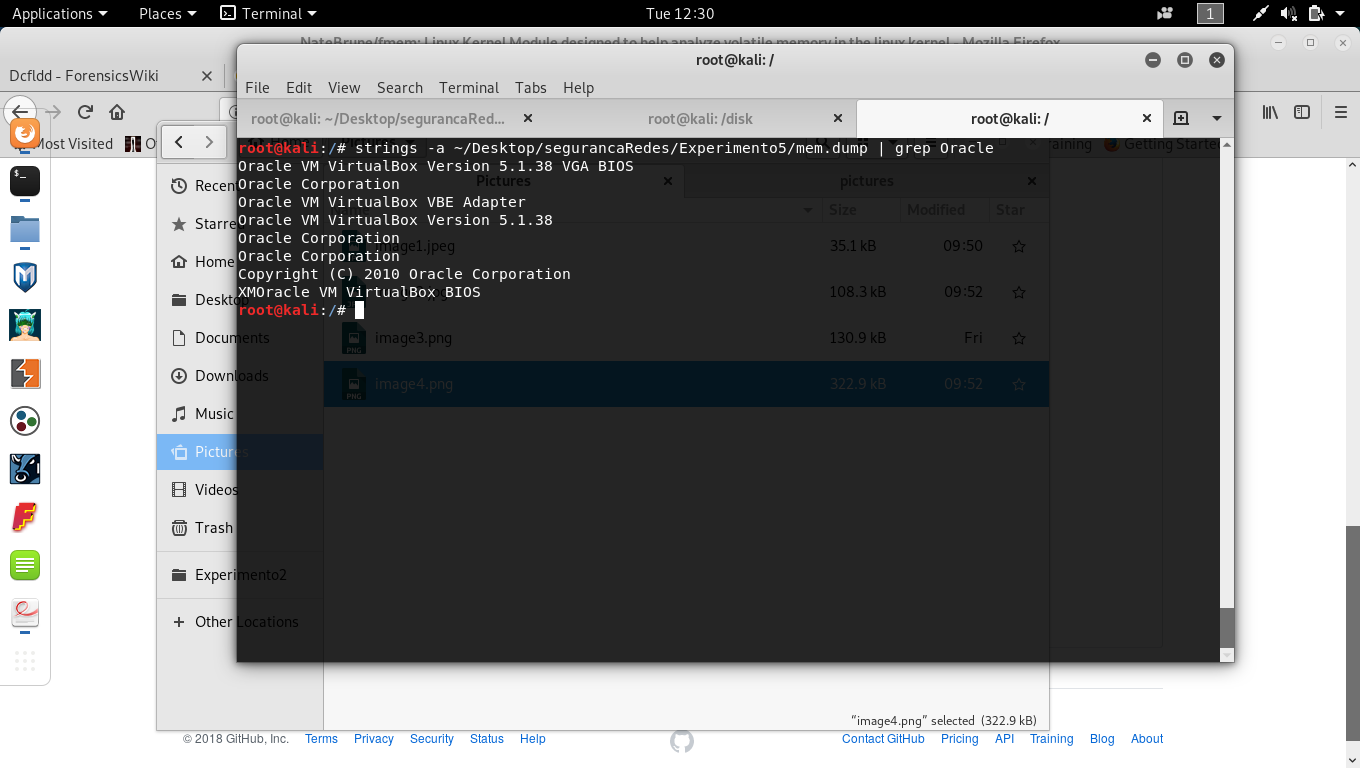
\includegraphics[width=\linewidth]{../pictures/dump_Oracle.png}
	\caption{Saída do dump da memória filtrado pela palavra 'Oracle'}
	\label{fig:memdump_oracle}
\end{figure}

\subsection{Carving Forensics (Extração)}
A extração é a prática de recompôr arquivos ou outros tipos de objetos de uma unidade de armazenamento. Todos os sistemas de arquivos possuem metadados, ou seja, dados que dizem respeito ao conteúdo ali presente. Na pior das situações será possível recompôr de um disco, sua hierarquia de arquivos, pelo menos. Essa é uma área computacional que poucos conhecem, e isso a deixa mais interessante ainda, pois criminosos não tomam tanto cuidado quanto deveriam aos descartar as evidências computacionais de seus crimes.
O processo de extração/'carving' requer conhecimentos em áreas como sistemas de arquivos dos sistemas operacionais. Isso porque, ao realizar uma extração, deve se conhecer o padrão de armazenamento utilizado naquela unidade. Comumente são utilizados sistemas como, por exemplo: FAT16, NTFS, EXT3, EXT4, dentre outros. Apesar de que o procedimento em sí, não depende tanto do sistema de arquivos utilizado, o conhecimento ajuda no entendimento do contexto, caso haja algum erro, por exemplo.\par
\subsubsection{MagicRescue}
Como ferramenta de extração, foi utilizado o 'Magicrescue', nativa no ambiente Kali. Na figura 2, é possível ver como foi utilizada a ferramenta, e o que se esperar do resultado impresso na tela. O parâmetro '-d' especifica o diretório de destino dos arquivos que serão extraídos, enquanto que o parâmetro '-r' especifica a "receita" desses arquivos, dessa forma o programa saberá como procurar por esses arquivos. Assim, é visto uma resposta positiva impressa no terminal.

%Imagem
\begin{figure}[h!]
	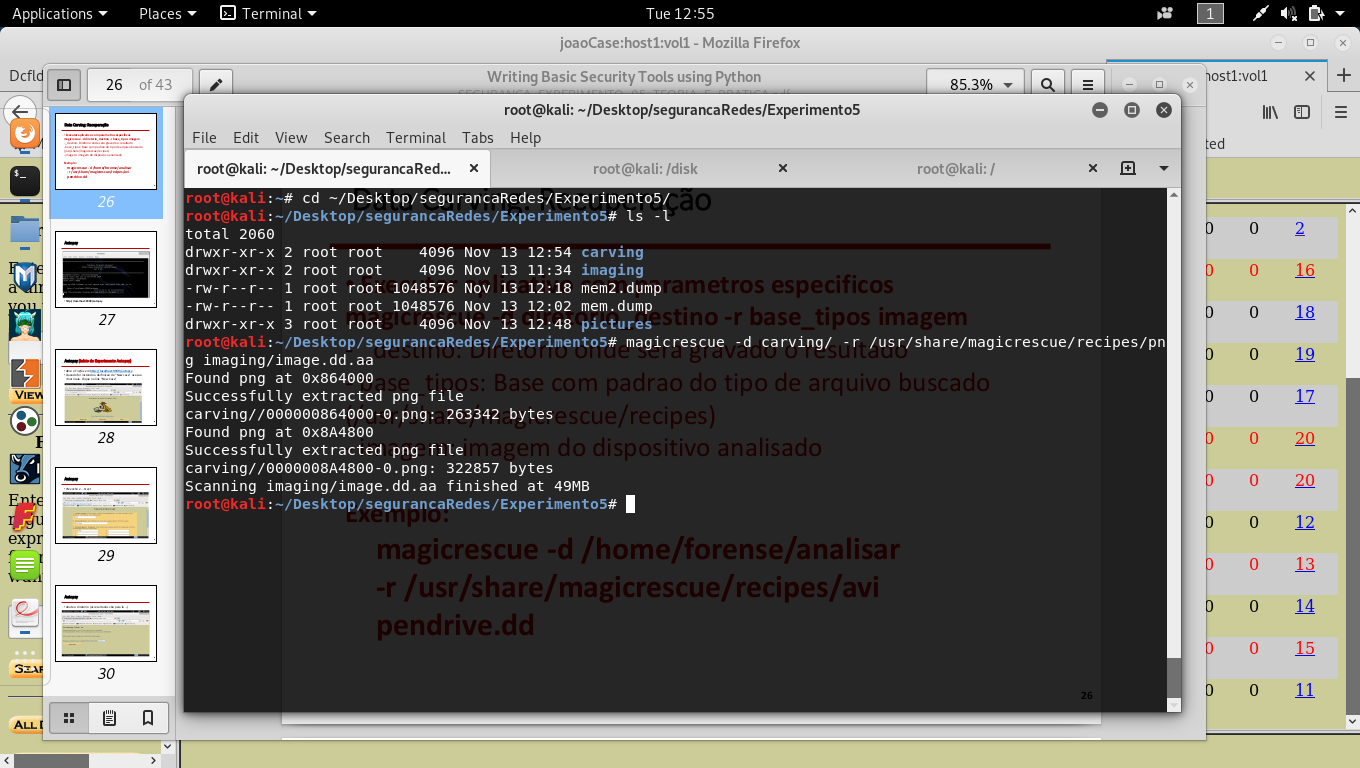
\includegraphics[width=\linewidth]{../pictures/carving/carving_output.png}
	\caption{Saída do magic rescue}
	\label{fig:magicrescue_carving}
\end{figure}

Como é visto na figura 3 logo abaixo, salvo no diretório 'carving' foram salvas exatamentes as imagens perdidas no disco apagado, foi possível extraí-las a partir, somente, da imagem do disco e uma receita de formato de arquivo. Infelizmente, o nome dos arquivos não pôde ser recuperado, porém veremos que existem outras ferramentas capazes de realizar esse trabalho.

%Imagem
\begin{figure}[h!]
	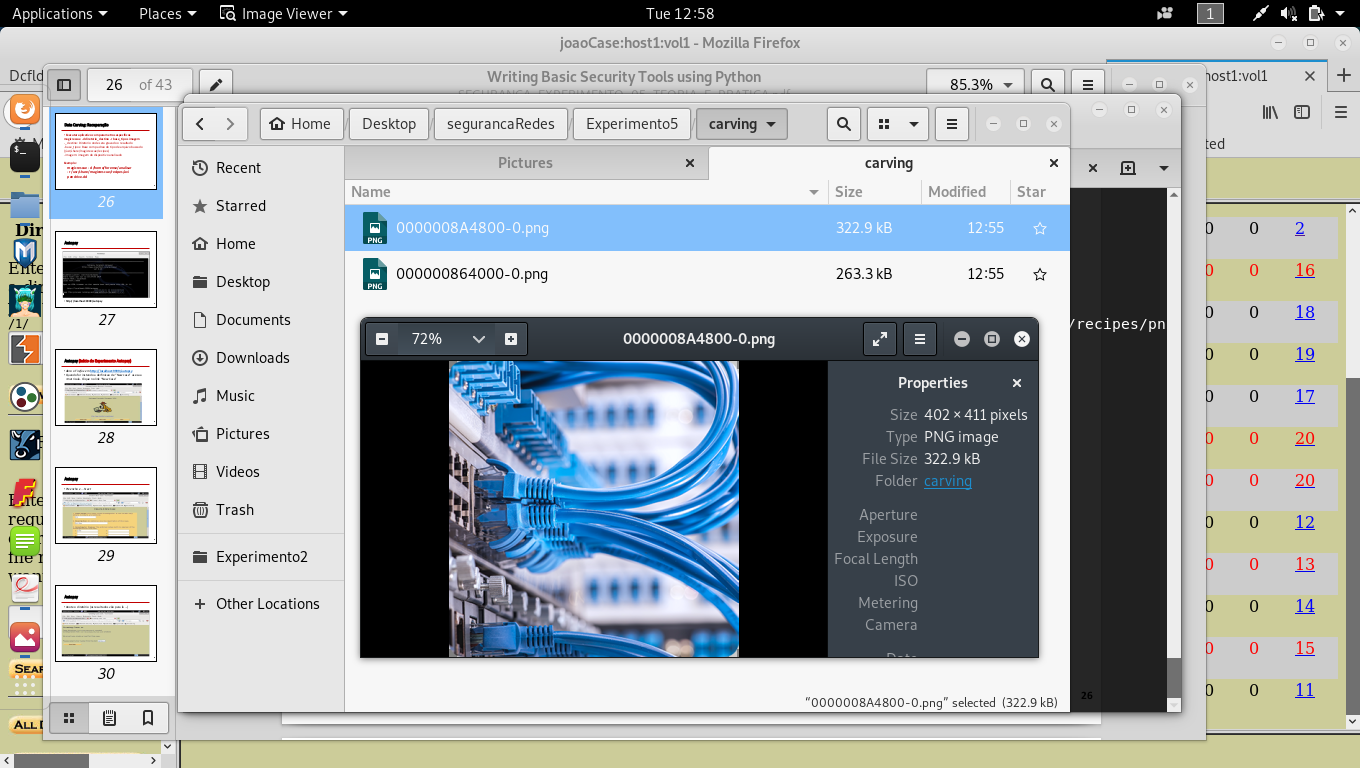
\includegraphics[width=\linewidth]{../pictures/carving/found_carved_images.png}
	\caption{Imagens recuperadas}
	\label{fig:carved_images}
\end{figure}

%Imagem
\begin{figure*}[p!t]
	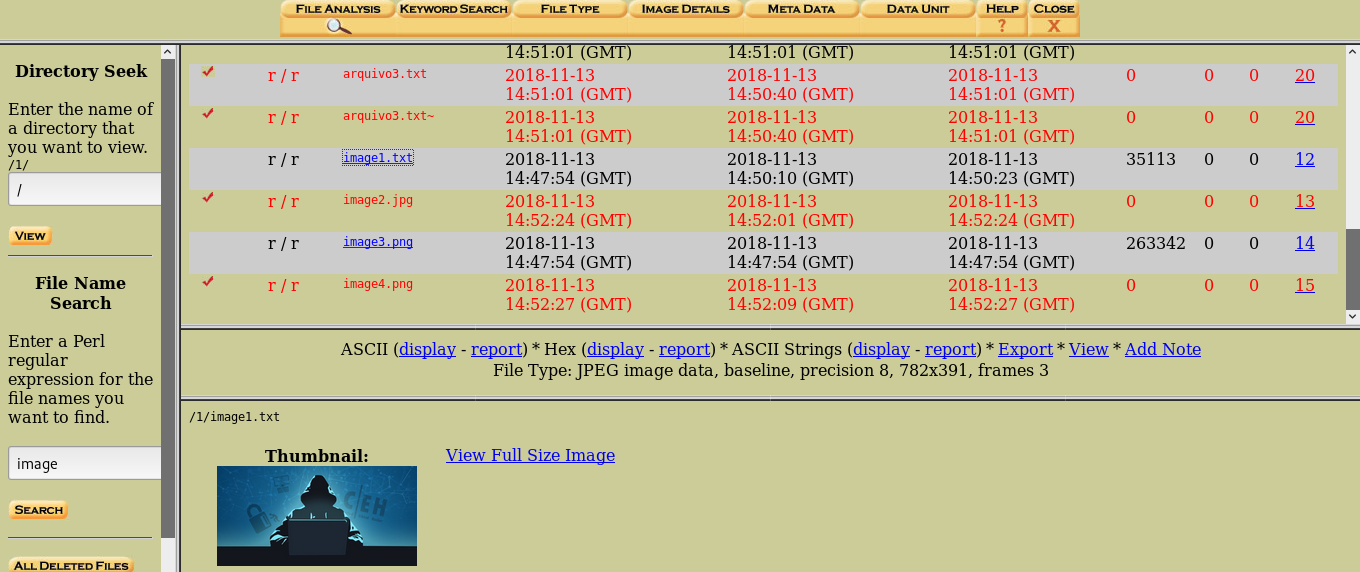
\includegraphics[width=\linewidth]{../pictures/autopsy/image_txt2.png}
	\caption{Arquivos recuperados}
	\label{fig:carved_files}
\end{figure*}


\subsubsection{Autopsy}
Foi utilizado o software Autopsy, já instalado por padrão na máquina Kali. É uma aplicação forense utilizada em diversas áreas de atuação, como, por exemplo, em investigações policiais e corporativas ou para fins militares, governamentais e acadêmicos. O Autopsy utiliza um sistema de 'casos', onde é necessário criá-los para iniciar uma investigação de um hospedeiro (\textit{host}). Um caso pode conter vários investigadores e vários hospedeiros, além disso, o autopsy funciona como um serviço na máquina, ou seja, dentro de uma organização, em sua rede interna, o Autopsy pode funcionar na porta 9999 de um servidor na LAN, possibilitando o acesso simultâneo de vários usuários. Nesse caso, foi criado um só investigador e um só hospedeiro com a imagem copiada do disco anteriormente, e foi adicionado também, o hash da imagem para verificar sua integridade. A imagem 4 mostra os arquivos recuperados da imagem, suas respectivas, permissões, horas de modificação e tamanhos. Além de todas essas informações, também é possível ver arquivos deletados, ou seja, deletar arquivos de um disco de armazenamento definitivamente não é suficiente para destruí-lo.


\subsubsection{p0f}
Investigações forenses não só são compostas de coleta de dados armazenados e estáticos, mas também dados que trafegam na rede. Será utilizado o p0f para analisar o tráfego TCP na máquina local. O p0f funciona como um "sniffer". Na figura 5 abaixo é possível ver um exemplo de captura de pacotes TCP em uma simples requisição HTTP.

%Imagem
\begin{figure}[h!]
	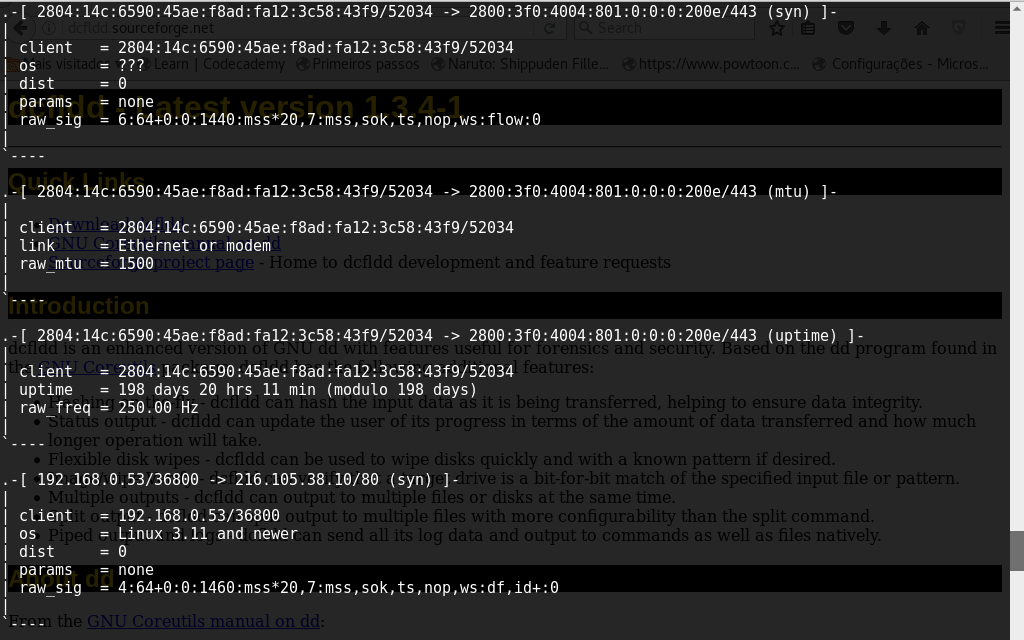
\includegraphics[width=\linewidth]{../pictures/p0f_tcp_packet.png}
	\caption{p0f capturando tráfego TCP}
	\label{fig:tcp_traffic}
\end{figure}


\section{Conclusion}
O hash criado no processo de cópia/coleta é feito por motivos de segurança. É necessário haver um método de verificação da imagem que está sendo analisada, afinal, quem poderá confirmar diante de um tribunal da corte se a evidência não foi adulterada, se é legítima? Além de que, hashs são extremamente convenientes de se trabalhar com, pela sua leveza e eficiência. Sim, é um algorítmo computacional unidirecional confiável, porém será suficiente para garantir a integridade da evidência? Essa é uma grande discussão na área forense, argumenta-se que da mesma forma que a imagem em questão pode ser corrompida e inválida, também pode ser o hash. Imaginando uma situação hipotética, onde ambos a imagem e o hash foram corrompidos pela mesma pessoa, ao serem analisados, teoricamente formam uma combinação "válida". Deve-se, portanto, aumentar a segurança nesse processo de validação da imagem. Com essa situação em mente, deve haver uma entidade confiável no meio de todo esse processo, como uma entidade certificadora no mundo web, análogamente. Essa mesma entidade, deve ser a responsável pela validação dos hashs, mantendo consigo uma base de dados confiável de todos os hashs que podem ser utilizados em tribunal. Dessa forma, partindo do pressuposto que essa entidade é 100\% confiável, é possível confirmar a integridade da evidência.



\begin{thebibliography}{1}

\bibitem{significado}
https://www.significados.com.br/forense/
\bibitem{rastros_virtuais}
https://www.contabeis.com.br/artigos/5035/seguindo-os-rastros-virtuais-computacao-forense/
\bibitem{digital}
https://en.wikipedia.org/wiki/Digital-forensicsForensic-data-analysis
\bibitem{dcfldd}
http://dcfldd.sourceforge.net/


\end{thebibliography}



\end{document}


